\documentclass{egpubl}
\usepackage{eurovis2021}

% --- for  Annual CONFERENCE
% \ConferenceSubmission   % uncomment for Conference submission
% \ConferencePaper        % uncomment for (final) Conference Paper
% \STAR                   % uncomment for STAR contribution
% \Tutorial               % uncomment for Tutorial contribution
% \ShortPresentation      % uncomment for (final) Short Conference Presentation
% \Areas                  % uncomment for Areas contribution
% \MedicalPrize           % uncomment for Medical Prize contribution
% \Education              % uncomment for Education contribution
% \Poster                 % uncomment for Poster contribution
% \DC                     % uncomment for Doctoral Consortium
%
% --- for  CGF Journal
% \JournalSubmission    % uncomment for submission to Computer Graphics Forum
% \JournalPaper         % uncomment for final version of Journal Paper
%
% --- for  CGF Journal: special issue
% \SpecialIssueSubmission    % uncomment for submission to , special issue
\SpecialIssuePaper         % uncomment for final version of Computer Graphics Forum, special issue
%                          % EuroVis, SGP, Rendering, PG
% --- for  EG Workshop Proceedings
% \WsSubmission      % uncomment for submission to EG Workshop
% \WsPaper           % uncomment for final version of EG Workshop contribution
% \WsSubmissionJoint % for joint events, for example ICAT-EGVE
% \WsPaperJoint      % for joint events, for example ICAT-EGVE
% \Expressive        % for SBIM, CAe, NPAR
% \DigitalHeritagePaper
% \PaperL2P          % for events EG only asks for License to Publish

% --- for EuroVis 
% for full papers use \SpecialIssuePaper
% \STAREurovis   % for EuroVis additional material 
% \EuroVisPoster % for EuroVis additional material 
% \EuroVisShort  % for EuroVis additional material

% !! *please* don't change anything above
% !! unless you REALLY know what you are doing
% ------------------------------------------------------------------------


\usepackage[T1]{fontenc}
\usepackage{dfadobe}


% \usepackage{cite}  % comment out for biblatex with backend=biber
% ---------------------------
\biberVersion
\BibtexOrBiblatex
\usepackage[backend=biber,bibstyle=EG,citestyle=alphabetic,backref=true,url=false]{biblatex}
%\addbibresource{egbibsample.bib}

\renewbibmacro*{doi+eprint+url}{%
    \printfield{doi}%
    \newunit\newblock%
    \iftoggle{bbx:eprint}{%
        \usebibmacro{eprint}%
    }{}%
    \newunit\newblock%
    \iffieldundef{doi}{%
        \usebibmacro{url+urldate}}%
        {}%
    }

\addbibresource{GeoVis.bib}

\newcommand{\citetitlea}[1]{\citefield{#1}{title}}

% ---------------------------  
\electronicVersion
\PrintedOrElectronic
% for including postscript figures
% mind: package option 'draft' will replace PS figure by a filename within a frame
\ifpdf \usepackage[pdftex]{graphicx} \pdfcompresslevel=9
\else \usepackage[dvips]{graphicx} \fi

\usepackage{egweblnk}
% end of prologue

\usepackage{float,hhline,hyperref,array,tabulary,tabularx,etoolbox,multirow}

% code listing
\usepackage{listings}
\lstdefinestyle{customc}{
  belowcaptionskip=1\baselineskip,
  breaklines=true,
  xleftmargin=\parindent,
  language=C,
  showstringspaces=false,
  basicstyle=\footnotesize\ttfamily,
  keywordstyle=\bfseries\color{green!40!black},
  commentstyle=\itshape\color{purple!40!black},
  identifierstyle=\color{blue},
  stringstyle=\color{orange},
}

\lstdefinestyle{customasm}{
  belowcaptionskip=1\baselineskip,
  xleftmargin=\parindent,
  language=[x86masm]Assembler,
  basicstyle=\footnotesize\ttfamily,
  commentstyle=\itshape\color{purple!40!black},
}

\lstset{escapechar=@,style=customc}

\usepackage{dblfloatfix}

\usepackage[table, dvipsnames]{xcolor}

\usepackage{multicol}

\author[Q. Wang \& R. S. Laramee]
{\parbox{\textwidth}{\centering Q. Wang
  and R. S. Laramee
    }
    \\
\parbox{\textwidth}{\centering School of Computer Science, University of Nottingham, UK}
}

\title{GHRVis:}

\begin{document}

\pagestyle{plain}

% auto labeling of sections
\let\origsection=\section
\renewcommand\section[1]{\origsection{#1}\label{sec:{#1}}}

\let\origsubsection=\subsection
\renewcommand\subsection[1]{\origsubsection{#1}\label{subsec:{#1}}}

\let\origsubsubsection=\subsubsection
\renewcommand\subsubsection[1]{\origsubsubsection{#1}\label{subsubsec:{#1}}}

\newcommand{\figureref}[1]{Figure \ref{#1}}
\newcommand{\tableref}[1]{Table \ref{#1}}
\newcommand{\phantomref}[1]{$\hyperref[#1]{\ref{#1}}$}

% Bob's dream paragraph style
\newcommand{\bobgraph}[1]{ \noindent\textbf{#1} \phantomsection \label{bobgraph:{#1}}}

\definecolor{Mycolor1}{HTML}{4C5866} %#4C5866
\definecolor{Mycolor2}{HTML}{A6B6D2} %#A6B6D2
\definecolor{Mycolor3}{HTML}{67daff} %#67daff
\definecolor{Mycolor4}{HTML}{F7F7FE} %#F7F7FE
\definecolor{Mycolor5}{HTML}{666ad1} %#666ad1
\definecolor{Mycolor6}{HTML}{ffbb93} %#ffbb93
\newcommand{\mycolorbox}[2]{\begingroup\setlength{\fboxsep}{2pt}\colorbox{#1}{#2}\endgroup}

% table cite
\newcommand{\citea}[1]{\citeauthor{#1}\cite{#1}}

% customized table headers
\newcommand{\theaderR}[1]{\multicolumn{1}{c|}{\cellcolor{Mycolor3} \textbf{\rotatebox{90}{#1 \phantom{-} }}}}
\newcommand{\theaderP}[1]{\cellcolor{Mycolor3} \textbf{#1}}

\newcommand{\note}[1]{\textcolor{blue}{#1}}

\newcommand{\expertcomment}[1]{\textit{``#1''}}

\newcommand{\task}[1]{\textbf{T#1}}
\newcommand{\req}[1]{\textbf{R#1}}

\maketitle

\begin{abstract}

\end{abstract}

\section{Introduction and Motivation}

Cartograms are representations of hybrid geographical and abstract data based on a value-by-area mapping technique combining statistical and geographical information \cite{dent2009Cartography}. Various styles of cartograms have been proposed and implemented, covering applications such as urban planning \cite{harris2018Mapping, arranz-lopez2021Enduser}, natural hazard forecasting \cite{pappenberger2019Cartograms, park2020Flood}, conservation and environmental planning \cite{galluzzi2018Mapping, rocchini2019Cartogramming}, political and social demographics \cite{breitzman2018Using, alieva2021How}, and public health decision making \cite{gao2020Visualising, sack2021Visualizing}.

Among the four types of cartograms categorized by \citea{nusrat2016State} (contiguous, non-contiguous, rectangular, and Dorling), a trade-off between types of accuracy is made (See \tableref{table:accuracy}). For this project we focus on non-contiguous cartograms like Demers cartograms, because they facilitate statistical comparison between regions and they can make good use of screen space. Building on Demers cartograms \cite{ian2002Cartogram}, we introduce and develop novel dynamic topological features, such as rivers, aiming to improve the readability and geographical accuracy without sacrificing statistical accuracy. We implement a new cartographic layout algorithm that includes these topological features into the layout of the nodes representing geographical regions. To minimize geographical errors and make efficient use of screen space, the algorithm also updates the position of rivers to accommodate the node layout. We then apply the algorithm to a real world case-study using an Electronic Health Records (EHR) dataset to evaluate of our algorithm. We also present a user study demonstrating its effectiveness.

Our contributions include:

\begin{itemize}
    \item A new variant of Demers cartograms that incorporates dynamic topological features to improve readability and recognizability,
    \item A novel layout algorithm that preserves node positions relative to dynamic topological features such as rivers,
    \item A user study evaluation of the technique with an application to EHRs.
\end{itemize}

One of the major challenges involved is how to develop a layout algorithm that handles different shapes. In other words, the layout algorithm is novel because it handles different types of nodes -- rectangular representing regions and polylines representing rivers. Another challenge we overcome in developing the algorithm is to resolve stalemate situations introduced by dynamic topological features while minimizing the geographical error.

\section{Related Work}
\begin{table*}[!tb]
	\centering
	\resizebox{\textwidth}{!}{
		\begin{tabulary}{\textwidth}{|*{3}{l|}r|c|}
			\hhline{~|*{3}{-}|~}
			\multicolumn{1}{c|}{\textbf{Literature}} &
			\textbf{Title} &
			\textbf{Geographic Region} &
			\textbf{Number of Nodes} &
			\multicolumn{1}{c}{\textbf{Year}} \\
			\hline
			
			% \citea{auber2007Geographical} & \citetitlea{auber2007Geographical} & US & 19 & 2007 \\
			% \hline
			\citea{warf2008Geography} & \citetitlea{warf2008Geography} & US & 3,142 & \citeyear{warf2008Geography} \\
			\hline
			\citea{sun2010Effectiveness} & \citetitlea{sun2010Effectiveness} & US, China & 34 - 49 & \citeyear{sun2010Effectiveness} \\
			\hline
			\citea{cruz2017Adapted} & \citetitlea{cruz2017Adapted} & Portugal & 2,882 & \citeyear{cruz2017Adapted} \\
			\hline
			\citea{tong2018cartograms} & \citetitlea{tong2018cartograms} & England & 209 & \citeyear{tong2018cartograms} \\
			\hline
			\citea{gao2020Visualising} & \citetitlea{gao2020Visualising} & China & 34 & \citeyear{gao2020Visualising} \\
			\hline
			\citea{nusrat2020Recognition} & \citetitlea{nusrat2020Recognition} & Portugal & 49 & \citeyear{nusrat2020Recognition} \\
			\hline
			



			% \multicolumn{1}{c|}{\textbf{Total unique papers: 51}} & 24&15&12& \multicolumn{1}{c}{}  \\
			% \hhline{~|*{3}{-}|~}

		\end{tabulary}
	}
	\caption{Discuss Demers cartogram}
	\label{table:challenge table}
\end{table*}

\section{Data Description}

Obtaining the heterogenous data can be challenging, especially when an Electronic Health Records (EHR) dataset is involved \cite{wang2021EHRa}. The data acquisition involves multiple steps. The first step is to obtain both geospatial boundaries and EHR data that match one another. The second step is to pre-process the EHR data to remove empty and erroneous values. The final step is to transform the data into a format that is suitable for visualization.

\subsection{Geospatial Data}

Geospatial boundaries, or shapefiles, were obtained from the following sources. After acquiring the shapefiles, we used QGIS \cite{qgisWelcome} to manually adjust projections and merge them into one shapefile. Finally, mapshaper \cite{blochMapshaper} is used to convert the merged shapefile into a TopoJSON \cite{TopoJSON} file to reduce the file size and improve the performance of our implementation.

{
\begin{figure}[tb!]
    \centering
    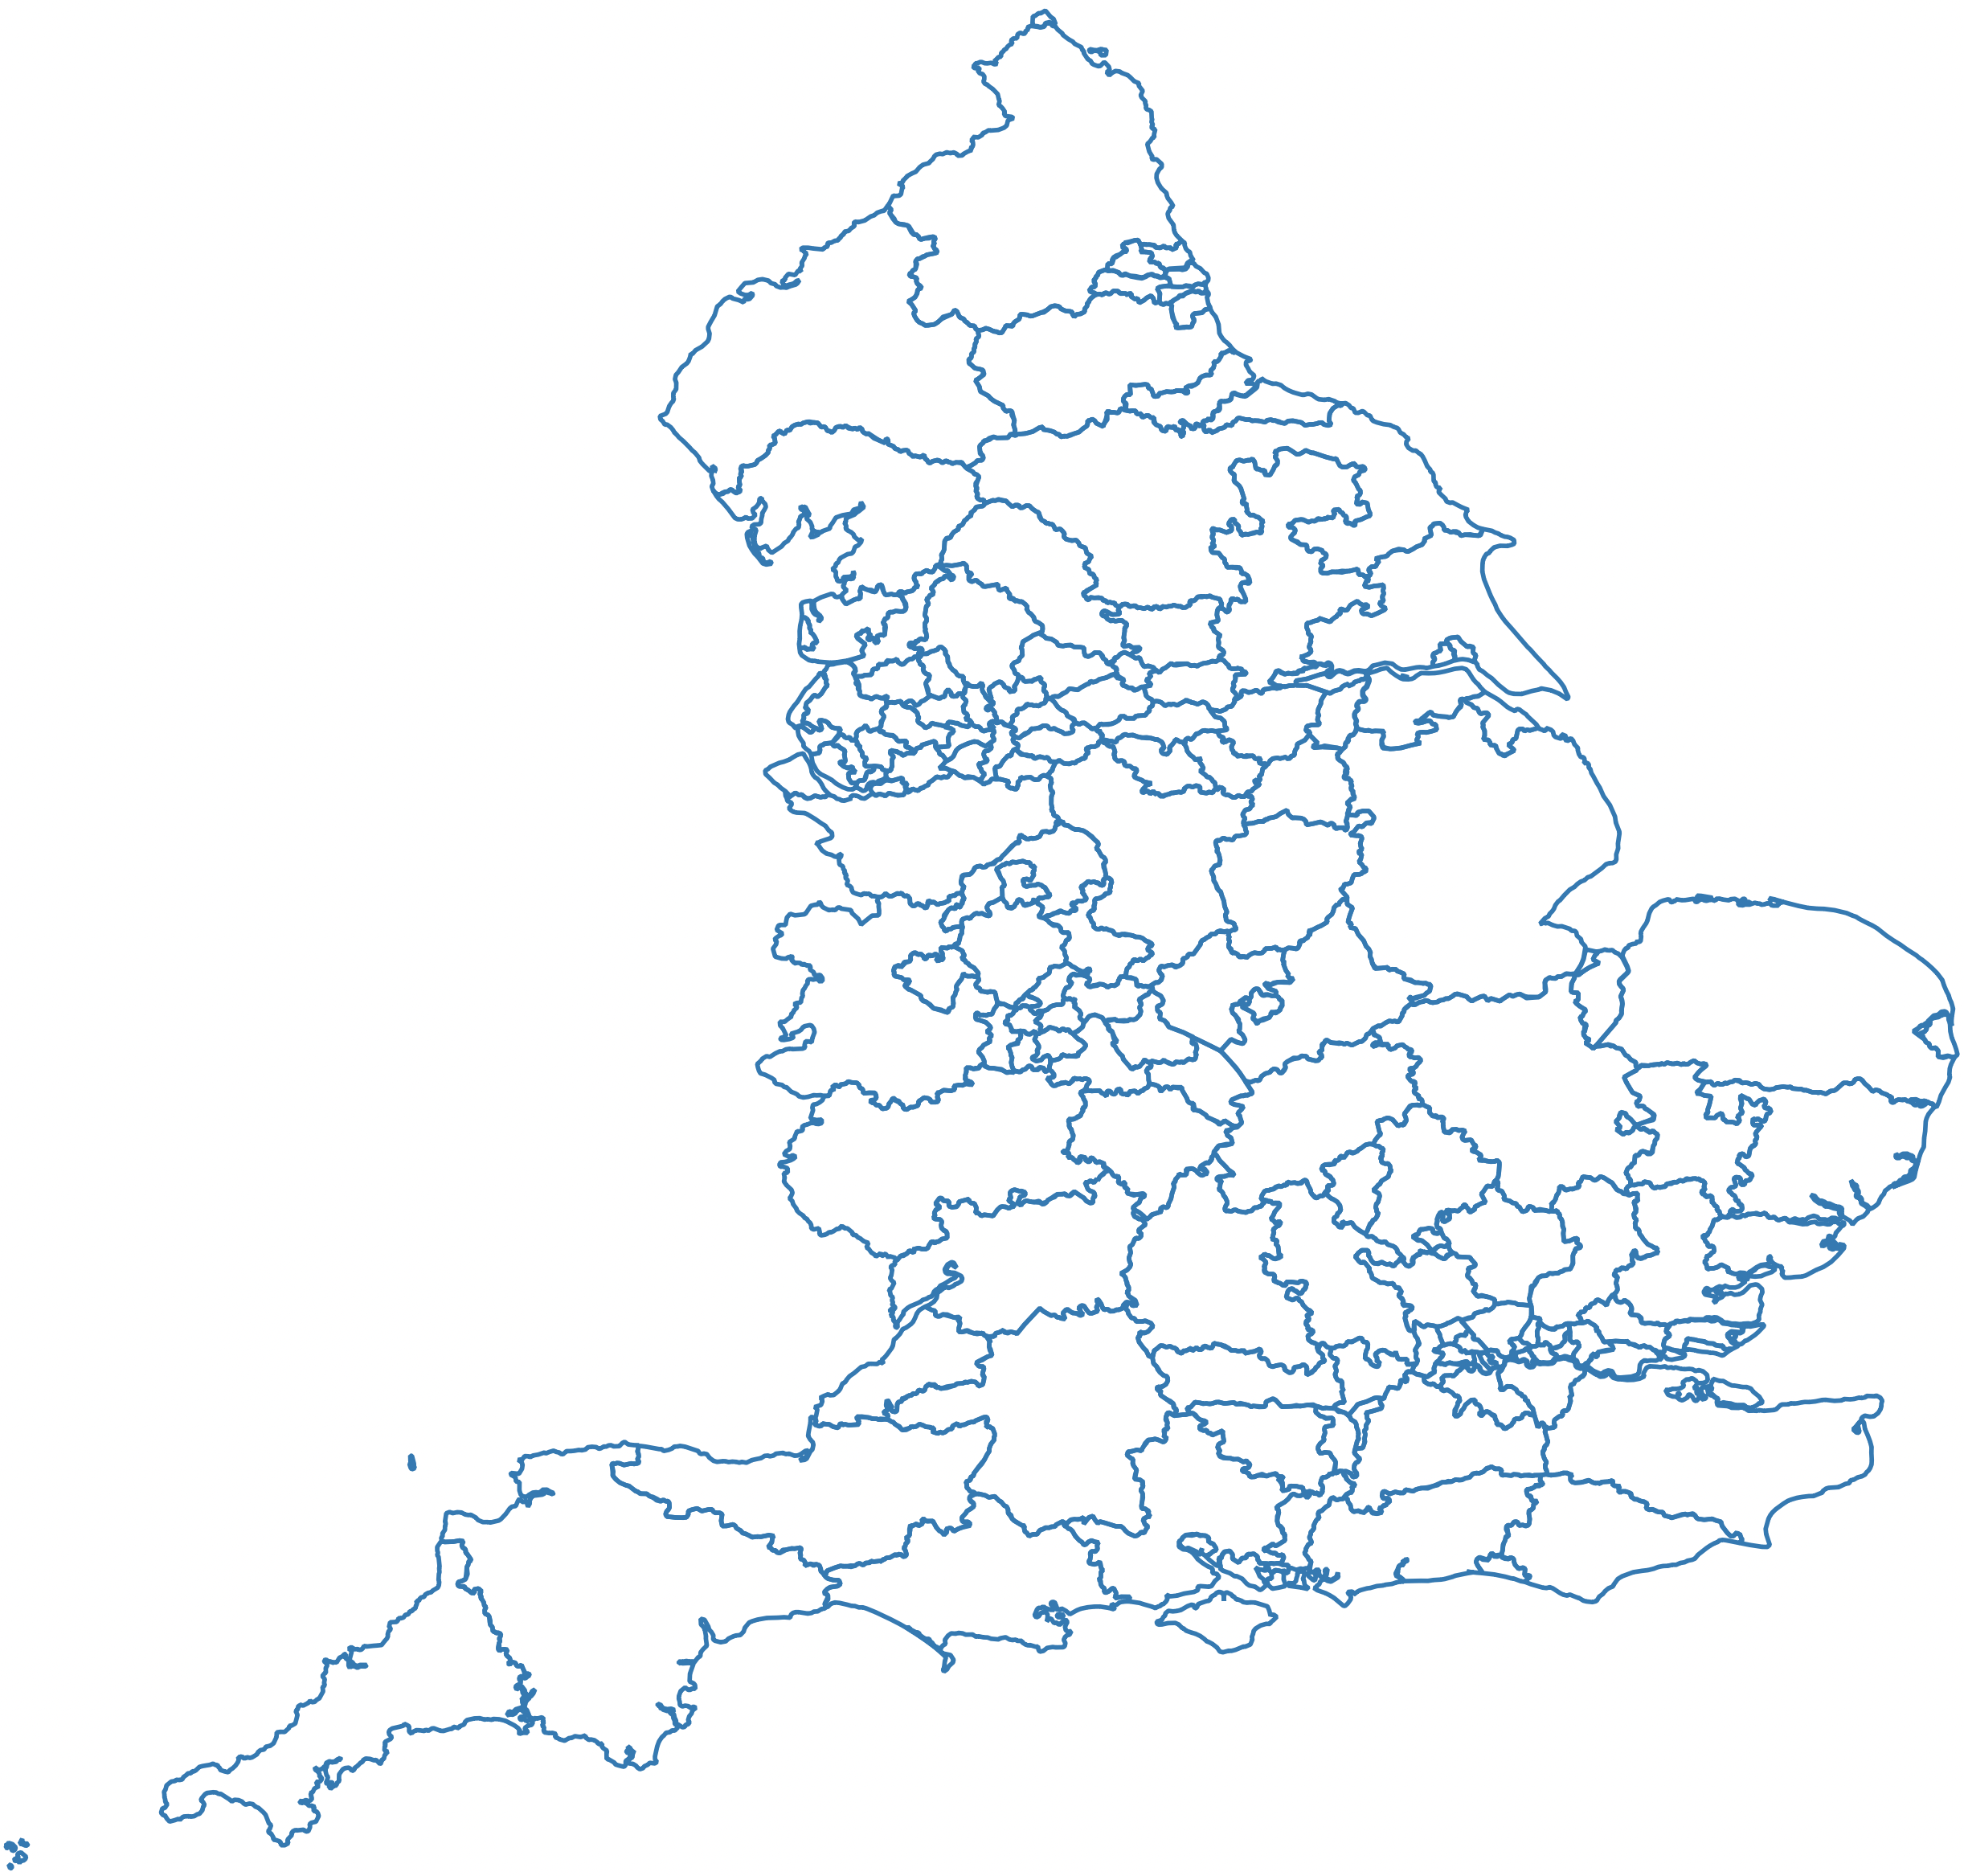
\includegraphics[width=0.6\columnwidth]{figure/ccg.png}
    \caption{A map of 135 CCGs in England as of 2020, obtained from the Open Geography portalx \cite{opengeographyportalxOpen}.}
    \label{fig:ccg}
\end{figure}
}

\subsubsection{Clinical Commissioning Groups Shapefile}

Clinical Commissioning Groups (CCGs) are the main geographic unit of the National Health Service (NHS) in the UK \cite{nhsNHS}. The number of CCGs changes over time due to the NHS re-organization. The most up-to-date shapefile is available from the Open Geography portalx \cite{opengeographyportalxOpen}. We decided to use the CCG shapefile from 2020 at the time of writing, because there is no public EHR data published based on the latest CCG re-organization that took place in 2021.

\subsubsection{River Features}

We used OpenStreetMap \cite{openstreetmapRelation} as our data source to obtain shapefiles for River Thames, River Trent and River Great Ouse in England. These rivers were chosen as they pass through regions with dense population, and provide informative geographical and topological cues. 

We first obtain a relation ID by searching for a river, e.g. River Thames, on OpenStreetMap. The relation ID is used to construct a query (See Listing~\ref{overpass}) which enables the user to download the entire river shapefile using Overpass Turbo \cite{overpassturboOverpass}.

\begin{lstlisting}[caption={The query that downloads the shapefile of River Thames from OpenStreetMap via the Overpass Turbo API.}, label={overpass},captionpos=b]
    relation(2263653);>>;
    out skel;
\end{lstlisting}

\subsection{EHR Data}

We obtained the Clinical Commissioning Group Outcomes Indicator Set (CCG OIS) from NHS Digital \cite{nhsdigitalClinical}. The OIS is a set of indicators that are used to measure the quality of care and the associated health outcomes in the NHS. Some datasets include:
\begin{itemize}
    \item Under 75 mortality
    \begin{multicols}{2}
        \begin{itemize}
            \item Cardiovascular disease
            \item Respiratory disease
            \item Liver disease
            \item Cancer
        \end{itemize}
    \end{multicols}
    \item Emergency hospital admission
        \begin{itemize}
            \item Stroke
            \item Alcohol-specific admission and readmission
            \item Coronary heart disease
            \item Readmissions within 30 days of discharge
            \item Children with lower respiratory tract infections
        \end{itemize}
\end{itemize}

For all datasets, a spreadsheet including the following data is provided:

\begin{itemize}
    \item Reporting period: Calendar year of registration
    \item Period of coverage: Start and end date or reporting period
    \item Breakdown: Organization type
    \item ONS code: UK Office for National Statistics CCG code
    \item Level: CCG Code
    \item Level description: CCG Name
    \item Gender
    \item Indicator value: Directly standardized mortality rate
    \item CI lower: lower 95\% confidence interval
    \item CI upper: upper 95\% confidence interval
    \item Denominator: The count of registered patients
    \item Numerator: Number of deaths
\end{itemize}

\section{GHRVis}

\subsection{VPSC}

\section{Evaluation}

\section{Limitations and Future Work}

\section{Conclusions}


\section{Acknowledgments}
This work is funded by the grant EP/S010238/2 from the Engineering and Physical Sciences Research Council (EPSRC). EPSRC is a British Research Council that provides government funding for grants to undertake research and postgraduate degrees in engineering and the physical sciences.

% reset \section command for section title "References"
\let\section=\origsection
\printbibliography

\end{document}

